\oldsection{Motivation and Objectives}

The goal of this project is to design a general-purpose multidimensional optimization algorithm based on genetic evolution. A major advantage of genetic algorithms is that they can optimize multidimensional objective functions, resulting in a series of Pareto-optimal 'individuals' from which the designer can choose the one best suited for some application. This document describes the successive improvements we made to our algorithm, and lists the results of each improvement. The algorithm is then applied to circuit design to obtain optimal parameters for the circuit to achieve certain specifications.

\oldsection{The algorithm}

The algorithm consists of several parts, described in the following sections.
\begin{enumerate}
	  \setlength\itemsep{0em}
\item initPopulation: initializes the population to random values. See \cref{initPopulation}.
\item evaluatePopulation: calculates the scores of each individual for each objective function. See \cref{evaluatePopulation}.
\item sortPopulation: sorts the population based on the objective function scores. Divides the population in ranks, where individuals in the same rank are pareto-equal to each other. A lower rank means Pareto-superior objective function scores. See \cref{sortPopulation}.
\item selectionTournament: selects parents out of the population. See \cref{selectionTournament}.
\item geneticOperators: generates children from the selected parents, by recombination or mutation. See \cref{geneticOperators}
\item cropPopulation: prevents the population size from growing. See \cref{cropPopulation}.
\item stopCriterion: determines when the algorithm converged. See \cref{stopCriterion}
\end{enumerate}

\subsection{InitializePopulation} \label{initPopulation}
This sets the population to a random matrix, where matrix elements are chosen randomly from a uniform distribution between 0 and 1. In order to make the population properties more general, more manageable, they are always scaled to the $[0,1]$ interval, except for the calculation of the objective scores (see \ref{evaluatePopulation}).
Ranks are set to 1, and crowding distance to 0 at initialization (see \ref{sortPopulation}).
For genetic algorithms, it's often better to have a better spread over the parameter space. We can assure this by choosing a pseudo-random initialization using the Sobol sequence \cite{sobol1976uniformly}.

\begin{figure}[h!]
	\centering
	\begin{subfigure}{.5\textwidth}
		\centering
		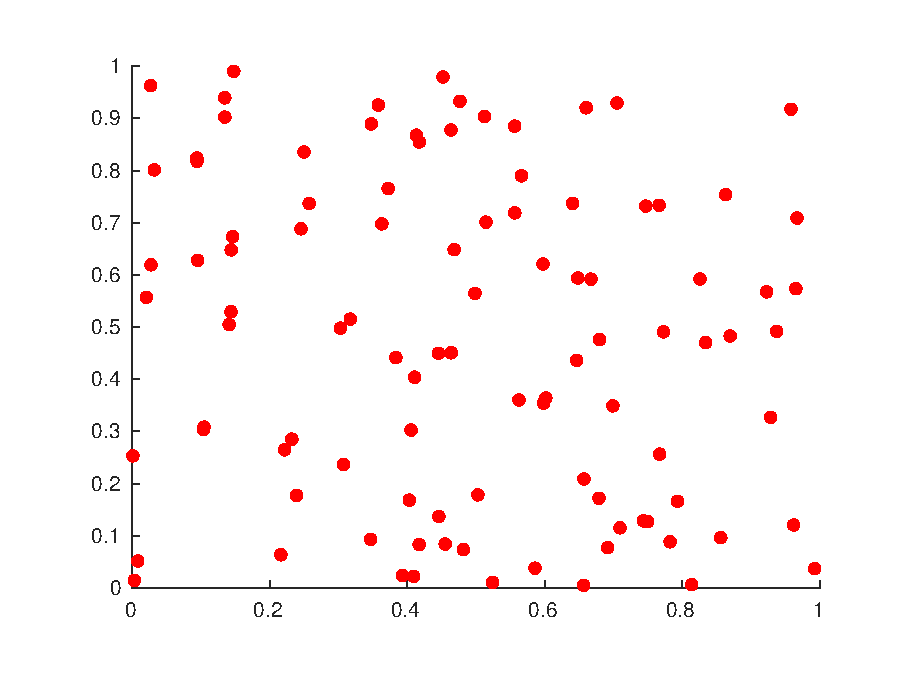
\includegraphics[width=0.8\textwidth]{images/randInit}
		\caption{distribution of a random population}
	\end{subfigure}%
	\begin{subfigure}{.5\textwidth}
		\centering
		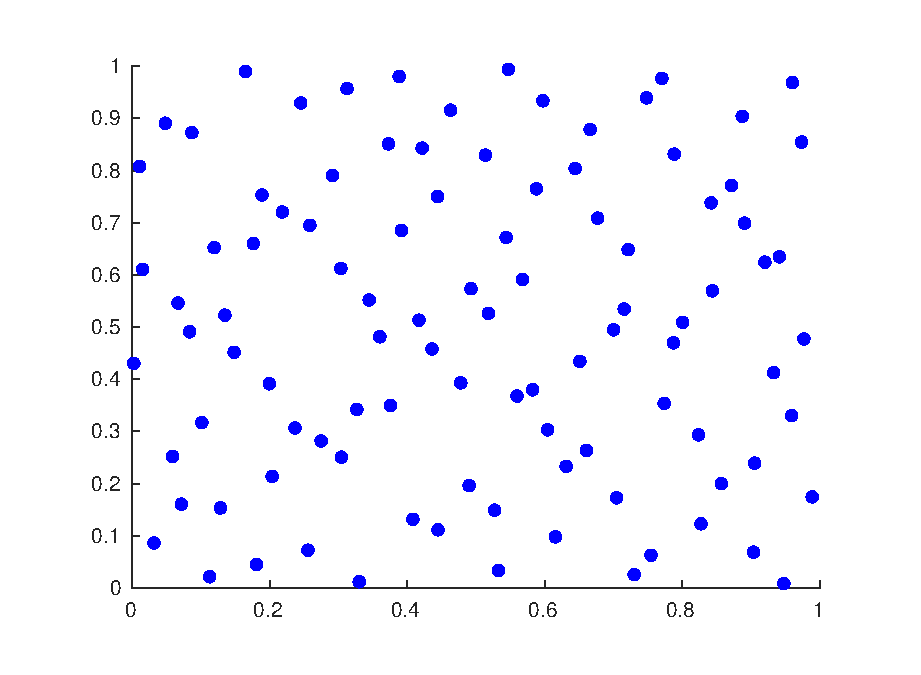
\includegraphics[width=0.8\textwidth]{images/sobolInit}
		\caption{distribution of a pseudorandom Sobel population}
	\end{subfigure}
\end{figure}

\subsection{EvaluatePopulation} \label{evaluatePopulation}
We save the rank and crowdingDistance columns, then unnormalize the population parameters in order to map from parameter space to objective space. The score for each objective function is calculated for each individual, and stored in columns V+1:V+M. The renormalized population parameters are stored in columns 1:V. 
In order to evaluate the population faster, the benchmark function is vectorized, so evaluatePopulation can run in parallel for the whole population.

\subsection{SortPopulation} \label{sortPopulation}
This function finds individuals that are on the same Pareto-optimal curve, and puts those in the same rank. The best rank is one, the worst one is rank three (more ranks would waste computation). The function has a slightly different version called sortPopulationCrowding which is called when all individuals in the population have rank 1. See subsection \ref{crowdingDistance}. 

\subsubsection{Ranking}
Individuals with low scores should be eliminated from the population. If the objective space is one dimensional, that can be easily done by sorting the scores in descending order and crop the ones in the bottom. When the objective space has two or more dimensions,  it is necessary to rank each individual based on their scores on all objective functions and give same rank to the individuals that lie on the same Pareto-optimal curve.

The ranking algorithm uses the concept of domination. An individual is dominated if there is another individual that has equal or better scores (better for at least one objective function ).

\subsubsection{Crowding Distance} \label{crowdingDistance}
The algorithm thus far doesn't give us good coverage of the whole Pareto-optimal solution space. It generates lots of individuals close together, which contain almost the same information. 

Crowding distance solves this problem. It's a measure of how close an individual is to other individuals in the parameter space. See \rref{NSGAII} for the algorithm of the crowding distance calculation. While sorting the population, crowding distance is taken into account, so that individuals with higher crowding distance are moved to the top within their rank.

% insert picture of sorted table with crowding distance

A problem arises however: when two individuals are close together both of their crowding distances will be low. If we then sort on crowding distance and remove the lowest scoring individuals, both might be removed. This is not the intention, as we want to keep one individual out of the group in our population. To prevent this, crowding distance is recalculated every time after an individual is removed from the population. This is done inside sortPopulationCrowding function. Effectively, this function sorts and crops simultaneously.\\
These changes slow down the algorithm, so we only do this after all individuals in the population have reached rank 1 (which means that we've most likely reached the Pareto-optimal curve). Theoretically the curve might be non-optimal while all individuals are rank 1, but in practice that is extremely unlikely to happen. Before reaching this point, we only calculate crowding distance once to save computation.

\begin{figure}[h!]
	\centering
	\begin{subfigure}{.5\textwidth}
		\centering
		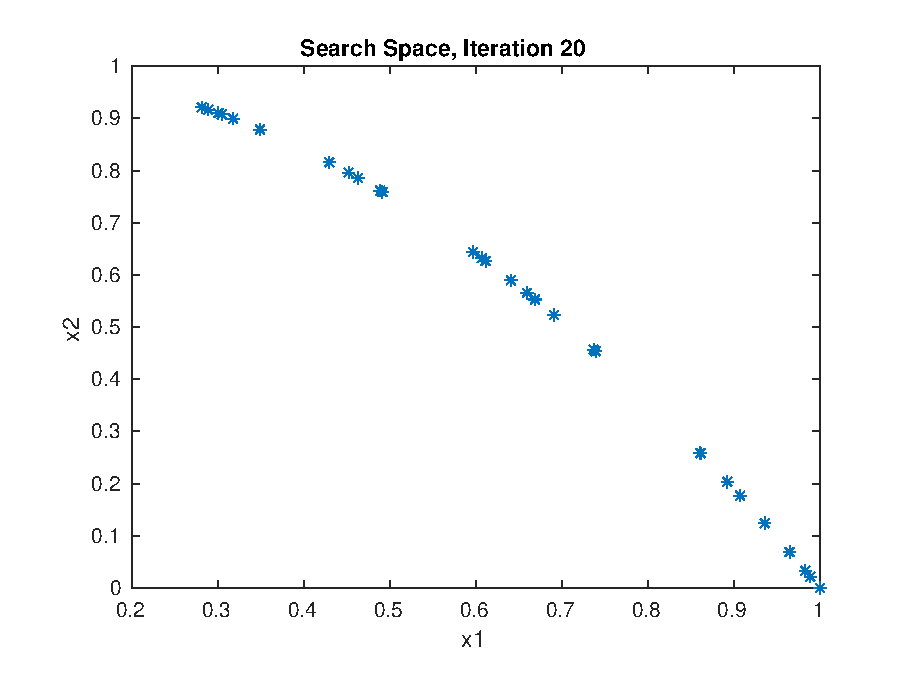
\includegraphics[width=0.9\textwidth]{images/noCrowding}
					\caption{convergence without crowding distance}
	\end{subfigure}%
	\begin{subfigure}{.5\textwidth}
		\centering
		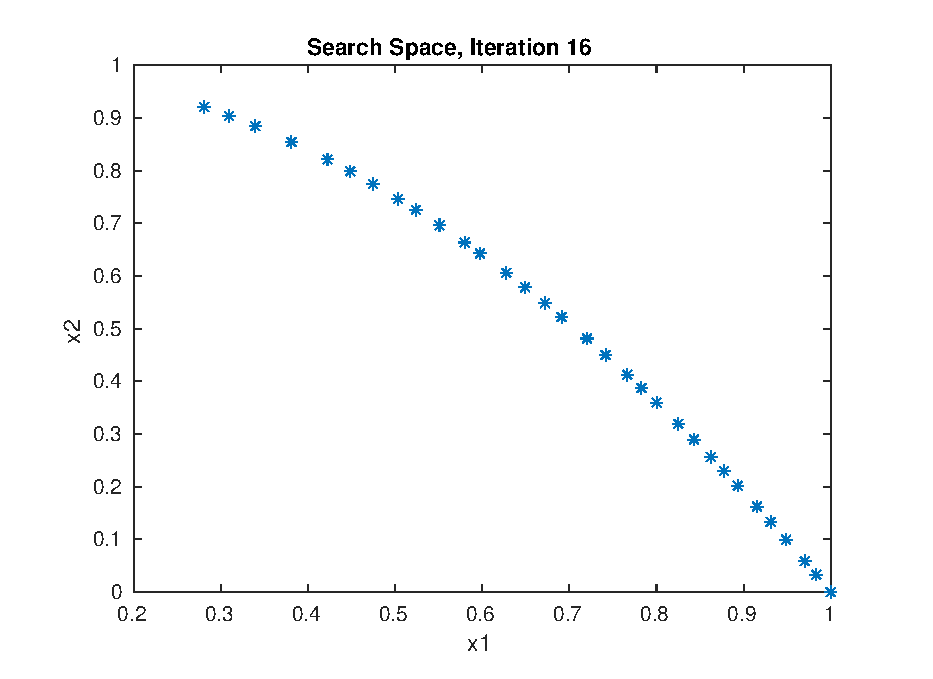
\includegraphics[width=0.9\textwidth]{images/niceCrowding}
		\caption{convergence with crowding distance}
	\end{subfigure}
	\label{fig:crowdingDistance}
\end{figure}

\subsection{selectionTournament} \label{selectionTournament}

This function takes number of parents (NP) as an input, select some parents from within the population, and returns a parent matrix as an output. The selection of parents is done with 'Tournament selection': two individuals are randomly selected and compared with each other. The one with better objective scores is added to the parent matrix if a predefined probability is satisfied. The procedure continues until NP parents are selected. 

Selection of best competitor is done by comparing their rank. In case their ranks are equal, the individual with higher crowding distance is favored as its genes are more valuable.

It may be mistakenly thought that selection of only the best NP individual of the population as parents is better. This is wrong, because it would converge to a local minimum instead of the global minimum. To find the global minimum, we need more randomness.

We had some ideas to try to increase the speed of convergence. We tried to select better parents, especially at the start of the algorithm when there are still lots of bad candidates.
First, make the probability of becoming a parent depend on rank. We chose the inverse of its rank to the power of four to prefer first-ranked individuals, and added a fixed bonus based on the crowding distance (prefer extreme individuals to increase search speed of parameter space).
Second, choose the elements with highest crowding distances as parents in the second phase (when the Pareto curve is reached). This would result in faster separation.
When we tested these changes, the first change actually degraded  convergence speed, possibly due to computational overhead. The second one did show some improvements.
\begin{table}[!htb]
	\caption{Summarizing table}
	\begin{minipage}{.5\linewidth}
		\caption{Large signal matching with real output inductors}
		\centering
		\begin{tabular}{ | l | l | l | }
			\hline
		 	 & Iterations & Runtime \\
		 	 \hline
			Avg &40.68	 &  0.67  \\
			Median &37.00 &  0.47\\
			Max &76.00	& 2.21 \\
			Std Dev & 12.87	&  0.48 \\
			\hline
		\end{tabular}
	\end{minipage}%
	\begin{minipage}{.5\linewidth}
		\centering
		\caption{Large signal matching with real output inductors}
		\begin{tabular}{ |l| l | l |}
			\hline
			& Iterations & Runtime \\
			\hline
			Avg    &      47.3   &   0.40 \\
			Median      &     43      &      0.34    \\
			Max		&	 158      &     1.9  \\
			Std Dev  &   25.2   &   0.34   \\
			\hline
		\end{tabular}
	\end{minipage} 
\end{table}


Simple binary tournament


First binary tournament, then select most crowding distanced
itAvg: 36.86|	 runTimeAvg:  0.55
itMedian: 34.00	|	 runTimeMedian:  0.49
maxIt: 82.00	|	 maxTime:  1.30 
stdIt: 13.52	|	 stdTime:  0.28 

select with randomness, most crowding distanced, but no cd in probability
itAvg: 39.54|	 runTimeAvg:  0.71
itMedian: 38.00	|	 runTimeMedian:  0.61
maxIt: 74.00	|	 maxTime:  2.07 
stdIt: 12.96	|	 stdTime:  0.48 





\subsection{GeneticOperators} \label{geneticOperators}

Genetic operations are used to create children from parents. There are two ways to create children: recombination and mutation. The recombination and mutation cannot happen at the same time. The probability of recombination (P) comes as an input and probability of mutation thus becomes (1-P).

\subsubsection{Recombination}

Recombination process should pass the properties of two randomly selected parents to the child. There are several approaches to do it. The most basic one is called "single-point crossover". Within this method, a split point is randomly chosen and the properties of the child until the split point are coming from the first parent while the remaining properties are coming from the second parent. This is easy to implement, but provides very little flexibility for the GA to find optimal combinations of properties. %a better explanation for the disadvantage of single-point crossover is needed

A better approach is to choose a random parent (out of the two) for each property. This is called "uniform crossover". A mixing ratio between parents is generated randomly between 1 and M. This ratio defines the number of properties that the first parent can pass to the child. The others will be selected from the second parent. Which properties are then chosen is determined randomly. After gene selection, a mutation is added (with standard deviation sd_mut_rec).
%\begin{figure}[h!]%
%	\centering
%	\centering
%	\includegraphics[width=0.6\textwidth]{images/recMutation}
%	\caption{Interpolatino method for recombination}
%	\label{fig:recMutationn}
%\end{figure}

%following paragraphs till mutation may be deleted or shortened
A different method uses interpolation. For each property, the values of the first and second parents define the initial interval boundaries. The interval is then scaled by some factor to allow for faster searching of the parameter space. 
% formula, graph of the interval, maybe an example matrix
%\begin{figure}[h!]
%	\centering%
%	\centering
%   \includegraphics[width=0.6\textwidth]{images/recInterpolation.eps}
%	\caption{Interpolatino method for recombination}
%	\label{fig:recInterpolation}
%\end{figure}
This approach blurs the boundaries between recombination and mutation as recombination through interpolation also allows the creation of children far away from parent's properties (which is what mutation is supposed to do). This is desirable at the start (because the parameter space is searched faster), but not when the population reached the Pareto curve. To solve this, we switch to different values for the parameters after reaching the Pareto curve. See \cref{hyperparameters}.

\subsubsection{Mutation}

In mutation, the child is generated only from one parent. The probability to be selected for each parent is 1/2. Mutation is defined as a Gaussian function centered to the parent. The standard deviation of the Gaussian function is taken as an input to the function.\\

Sometimes, it is possible to have properties outside 0-1 interval hence cutting those values are needed.

\subsection{cropPopulation} \label{cropPopulation}

After the children are added to the population, cropping is necessary to keep the population size same. Since the population is already sorted based on rank and crowding distance, cropping is done by selecting first N values and removing the rest from the matrix. 

\subsection{stopCriterion} \label{stopCriterion}

The algorithm needs to be stopped when all of the individuals are good enough. After all individuals are rank 1, the Pareto-optimal curve does not converge any further. It will rather start to spread the points on the curve so that each will have a high crowding distance. \\
One way to determine when the Pareto curve is reached is to look when all individuals have rank 1. This means no point is being dominated. In practice, this works very well. Theoretically it's possible that this happens when the population has not yet reached the Pareto curve, but this is extremely unlikely.
To determine the spreading we use the coefficient of variation of the crowding distance vector \cite{CV}. This is the standard deviation divided by the mean. Empirically, a value of 0.15 was found to give good spreading while maintaining convergence speed. However, the standard deviation doesn't consider extremities, so we add a check that the highest and lowest crowding distances have to be close to the median value. This means all points will have similar spreading.

\section{Determining hyperparameters} \label{hyperparameters}
The algorithm requires lots of hyperparameters: P, sd_mut, N, NP, NC. There are three ways to determine optimal values for these:
\begin{enumerate}
\item Manually: change values, observer convergence speed, and reiterate. This works reasonably well, but is a slow and time-consuming process.
\item Parameter Sweep: for each parameter, loop through values, and test convergence speed.
\item Genetic Optimization: use a genetic algorithm of which the parameters were manually determined to find optimal values for the GA.
\end{enumerate}
A set of parameters is evaluated by running the ZDT6 algorithm until convergence, or until 500 iterations have passed. To increase simulation speed, different sets are evaluated in parallel, and objective function and function evaluations are vectorized.

\subsection{Manual search}
For the recombination using interpolation, this resulted in:\\
N = 24;         % Population size
NP = 12;       % Size of the mating pool
NC = 24;       % Number of children generated by generation
P = 0.8;	% Recomination probability
sd_mut = 0.1; %standard deviation for mutation
These values result in the following convergence speed (calculated by running simulations until the average didn't change anymore):
\begin{table}[H]
\centering
\begin{tabular}{|l|c|c| }
\hline
& Number of Iterations	& Runtime \\
\hline
average    &      47.3   &   0.40 \\
median      &     43      &      0.34    \\
maximum		&	 158      &     1.9  \\
std dev  &   25.2   &   0.34   \\
\hline
\end{tabular}
\caption{convergence for manual hyperparameters}
\label{manualConvergence}
\end{table}
These values were used for the GA that ran genetic optimization of the parameters.

\subsection{Parameter Sweep}
A sweep was run over P, sd_mut, N, NP, NC. Since the parameter space is very large and each evaluation costs a lot of computation power (we test for convergence speed), the first sweep is very crude.
A second sweep can concentrate on the areas that show promising results.

\subsection{Genetic Optimization} 
In order to optimize the parameters of the PA, we write a function with fixed parameters (myOptimizeGA.m), which are determined manually.
The evaluation of the top-level population (containing GA parameters) happens through benchmark.m, where an extra case was added which calls myGAEvaluate.m.
This function runs a GA on ZDT6 until convergence or 500 iterations, and returns the number of iterations and the runtime, divided by N (as larger populations have a disadvantage due to the crowding distance calcuations after reaching the optimal curve, see \ref{crowdingDistance}). It also adds penalties to the runtime if the GA hasn't been able to converge.
To increase speed, vectorization and parallel execution (eg MATLAB's parfor) are used and some starting values are used in the initial population. \\

\section{Differential Pair} 

The genetic optimization was implemented to both single and double ended differential amplifiers. Initially power and gain bandwidth product are used as two dimensional objective space. Later, three dimensional objective space is also tried with the addition of area as the third objective. In all implementations, a good convergence curve is observed in which trade off between different design parameters are clearly visible. 

The circuit is simulated in Eldo. An interface function enabled the extraction of simulation results to Matlab. Output voltage is extracted from AC simulation. Magnitude and phase for each frequency for the output voltage is calculated. The gain is found as the magnitude of first index of the output voltage. The bandwidth is found as detecting -3dB crossing point (in other words, 70percent of the initial gain). If bandwidth cannot be detected, the BW is made equal to 1Hz. Furthermore, current drawn from the power supply is extracted from the DC simulation. The multiplication of this value and bias voltage are used to find power consumption.


\section{Future Improvements}
\section{Summary of  Achievements}\label{summary}

With our implementation, we managed to obtain pretty good results. 
